\ifx \mpreamble \undefined
\documentclass[12pt,a4paper]{article}
\usepackage{answers}
%\usepackage{microtype}
\usepackage[left=3cm,top=2cm,bottom=3cm,right=2cm,includehead,includefoot]{geometry}

\usepackage{amsfonts,amsmath,amssymb,amsthm,graphicx}
\usepackage[utf8]{inputenc}
\usepackage[T1]{fontenc}
\usepackage{ngerman}

\usepackage{pstricks}
\usepackage{pst-circ}
\usepackage{pst-plot}
%\usepackage{pst-node}

\ifx \envfinal \empty
\usepackage{pst-pdf}
\fi

\usepackage{booktabs}

% Muss als letztes eingebunden werden
%\usepackage[bookmarks=true,bookmarksnumbered,colorlinks=true,pdftitle={IPhO-Aufgaben},pdfstartview=FitH,pdfauthor={Pavel Zorin}]{hyperref}
\usepackage[bookmarks=false,pdftitle={IPhO-Aufgabensammlung},pdfstartview=FitH,pdfauthor={Pavel Zorin}]{hyperref}

%Times 10^n
\newcommand{\ee}[1]{\cdot 10^{#1}}
%Units
\newcommand{\unit}[1]{\,\mathrm{#1}}
%Differential d's
\newcommand{\dif}{\mathrm{d}}
\newcommand{\tdif}[2]{\frac{\dif#1}{\dif#2}}
\newcommand{\pdif}[2]{\frac{\partial#1}{\partial#2}}
\newcommand{\ppdif}[2]{\frac{\partial^{2}#1}{\partial#2^{2}}}
%Degree
\newcommand{\degr}{^\circ}
%Degree Celsius (C) symbol
\newcommand{\cel}{\,^\circ\mathrm{C}}
% Hinweis
\newcommand{\hinweis}{\emph{Hinweis:} }
% Aufgaben mit Buchstaben numerieren
\newenvironment{abcenum}{\renewcommand{\labelenumi}{(\alph{enumi})} \begin{enumerate}}{\end{enumerate}\renewcommand{\labelenumi}{\theenumi .}}
%%%%%%%%%% Skizzen %%%%%%%%%%%%
%\ifx \envfinal \empty
%%% Final
%\else
%%% Vorschau
%\fi

\def \mpreamble {}
\else
%\ref{test}
\fi
\ifx \envfinal \undefined


\newcommand{\skizze}[1]{
\begin{figure}
\begin{center}
#1
\end{center}
\end{figure}
}




%\documentclass[12pt,a4paper]{article}
\newcounter{numlabel}
\setcounter{numlabel}{0}

\newcommand{\problemlabel}{}
\newenvironment{problem}[2]{
\stepcounter{numlabel}
\renewcommand{\problemlabel}{Aufgabe \the\value{numlabel}: #1}
\subsubsection*{\problemlabel \emph{(#2 Punkte)}}
}{}
\newenvironment{solution}{\subsubsection*{\problemlabel}}{}
\newenvironment{expsolution}{\subsubsection*{\problemlabel}}{}

\begin{document}

\fi

\begin{problem}{Nachthimmel}{3}
Man nehme an, das Universum sei unendlich groß, auf großen Distanzen homogen mit Sternen gefüllt, isotrop und unendlich alt.
\begin{abcenum}
\item Wie hell ist der Nachthimmel unter diesen Annahmen?
\item Wie ändert sich diese Helligkeit, falls im Universum signifikant viele homogen verteilte interstellare Gaswolken entstehen?
\item Warum beobachtet man den beschriebenen Zustand nicht?
\end{abcenum}
\begin{solution}
\begin{abcenum}
\item In der Aufgabenbesprechung wurde behauptet, die Intensität sei unendlich groß, dies stimmt allerdings nur unter der Annahme, dass Sterne exakt punktförmig sind und trotzdem eine endliche Leistung abstrahlen. Wenn die Sterne eine endliche Ausdehnung besitzen, entspricht die Intensität der mittleren Farbtemperatur der Sterne.
\end{abcenum}
\end{solution}
\end{problem}


\begin{problem}{Schaerfentiefe}{4}
In einer Kamera wird ein Objekt mit einer Linse (Brennweite $f$) durch die Blende (Durchmesser $D$) auf die Filmebene abgebildet. Die Schärfentiefe ist die zulässige Verschiebung des Objektes entlang der optischen Achse, bei der sich das Bild um höchstens einen vorgegebenen Abstand $l$ verschiebt. Man bestimme diese in Abhängigkeit von den auftretenden Parametern.

\begin{solution}
\[
\Delta g = \frac{2 l g^2}{D f}
\]
\end{solution}
\end{problem}


\begin{problem}{Schmelzen von Eis}{5}
\skizze{
\begin{pspicture}(-2.75,-2.5)(2.75,2.5)
%\pscircle(0,2){2}
%\psarc{|-|}(0,0){2}{0}{180}
%\psarc{|-|}(0,0){2}{180}{360}
\pscircle(0,0){2}
\psellipticarc[linestyle=dashed,linewidth=2\pslinewidth](0,0)(2,1){0}{180}
\psellipticarc[linewidth=2\pslinewidth](0,0)(2,1){180}{360}
\pscircle(0,0){1.5}
\psellipticarc[linestyle=dashed](0,0)(1.5,0.75){0}{180}
\psellipticarc(0,0)(1.5,0.75){180}{360}

\rput{120}(0,0){
\psline{->}(0,0)(2,0)
\rput{-120}(2.3,0){$r_2$}
}
\rput{160}(0,0){
\psline{->}(0,0)(1.5,0)
\rput{-160}(0.6,0.4){$r_1$}
}

\rput(2,1.5){$20 \cel$}
\rput(2,-1.5){$15 \cel$}
\end{pspicture}
}
In einem evakuierten kugelförmigen Isoliergefäß mit dem inneren Radius $r_1 = 5 \unit{cm}$ und dem äußeren Radius $r_2 = 10 \unit{cm}$ befinden sich jeweils $100 \unit{g}$ Wasser und Eis (spezifische Schmelzwärme $334 \unit{J/g}$) im Gleichgewicht. Die obere Hälfte der Außenhülle hat die konstante Temperatur $20 \cel$, die untere Hälfte ist von dieser isoliert und wird bei $15 \cel$ gehalten. Wie lange dauert es, bis das gesamte Eis im Gefäß geschmolzen ist?
\begin{solution}
An die innere Kugel abgestrahlte Leistung:
\[
P = 2 \pi r_1^2 (T_1^4+T_2^4-2 T_0^4) \sigma
\]
\[
t = \frac{m_\mathrm{Eis} \lambda_\mathrm{Eis}}{P} \approx 3.3 \unit{h}
\]
\end{solution}
\end{problem}


\begin{problem}{Garnrolle}{4,5}
\skizze{
\begin{pspicture}(-2.75,-1.9)(2.75,1.9)
\pscircle(0,0){1.8}
\pscircle(0,0){1}
\psline(-3,-1.8)(3,-1.8)
\rput{30}(0,0){
\psline{->}(0,0)(0,-1)
\psline{->}(0,-1)(2.5,-1)
\rput{-30}(2.25,-0.6){$F$}
\rput{-30}(0.25,-0.5){$r$}
\rput{-30}(0,-1){
\psline[linestyle=dashed](0,0)(1.5,0)
\psarc(0,0){0.5}{0}{30}
\rput(0.75,0.2){$\alpha$}
}
}
\psline{|<->}(-2.25,0)(-2.25,-1.8)
\uput[l](-2.25,-0.9){$R$}
\end{pspicture}
}
An dem Ende des auf eine Garnrolle aufgewickelten masselosen Fadens wird mit konstanter Kraft $F$ gezogen. Welcher Drehmoment wirkt auf die Rolle? In welche Richtung wird sich die Rolle bewegen, wenn sie nicht rutscht?
\begin{solution}
Drehmoment um den Auf\/lagepunkt:
\[
\vec M = \vec R_F \times \vec F =
\begin{pmatrix} r \sin \alpha \\ R - r \cos\alpha \\ 0 \end{pmatrix}
\times
\begin{pmatrix} F \cos \alpha \\ F \sin\alpha \\ 0 \end{pmatrix}
\]
\[
M_z = F (r - R \cos\alpha)
\]
Je nach Vorzeichen des Drehmoments bewegt sich die Rolle nach links (positiv) oder nach rechts (negativ).
\end{solution}
\end{problem}


\begin{problem}{Resonante Tunneldiode}{6,5}
\skizze{
\psset{unit=1.25cm}
\begin{pspicture}(-1,-0.5)(4.5,3.5)
\psline{->}(0,0)(4,0)
\uput[275](4,0){$\mathrm{Ort}$}
\psline{->}(0,0)(0,3)
\uput[30](0,3){$\mathrm{Energie}$}

\psline(0,1.5)(1,1.5)(1,2.5)
\psline(1.5,2.5)(1.5,1)(2.5,1)(2.5,2.5)
\psline(3,2.5)(3,0.5)(4,0.5)

\psline{|->}(1.25,1.5)(1.25,1)
\uput[l](1.25,1.25){$\alpha e U$}

\psline{|->}(2.75,1.5)(2.75,0.5)
\uput[l](2.75,0.75){$e U$}

\psline[linestyle=dashed](0,2.2)(1,2.2)

\psline[linewidth=0.05](1.5,2)(2.5,2)
\psline{->}(0.5,2)(3.5,2)

\uput[270](2,2){$E_1$}
\uput[90](2,2){$\vdots$}

\psline{|-|}(1.5,0)(2.5,0)
\uput[270](2,0){$l$}
\end{pspicture}
}
In einer Tunneldiode sind die Anschlüsse durch zwei Potentialbarrieren im Abstand $l$ voneinander getrennt. Durch die Quantisierung möglicher Energieniveaus in dem dazwischenliegenden Potentialtopf können die Elektronen genau dann besonders leicht durch das System tunneln, wenn diese einen stationären Zustand im Potentialtopf einnehmen können. Wenn man an die Diode eine Spannung anlegt, wird diese in einem konstanten, diodenspezifischen Verhältnis aufgeteilt, wodurch die günstigen Energieniveaus relativ zu den ankommenden Elektronen verschoben werden können.
\begin{abcenum}
\item Welche Wellenlängen können die Elektronen im Potentialtopf haben? Wie groß sind die zugehörigen Energien? \hinweis Die effektive Masse des Elektrons $m^*$ kann sich i.\ A. von der freien Elektronenmasse $m_e$ unterscheiden.
\begin{figure}[h]
\centering
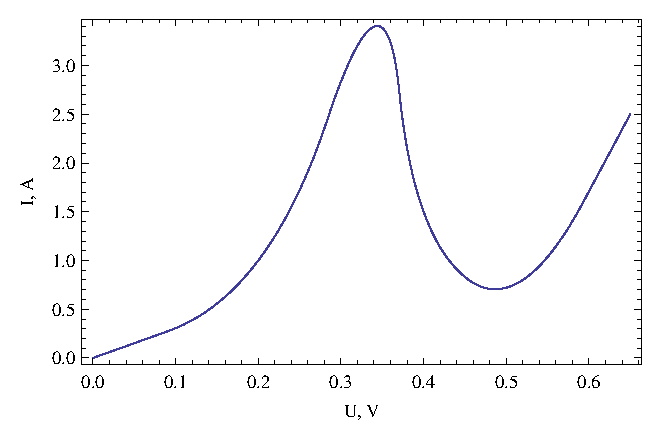
\includegraphics{bilder/resonante_tunneldiode_1.eps}
\end{figure}
\item Die Abbildung zeigt das U-I-Diagramm einer GaAs-RTD mit $l=5 \unit{nm}$. Für diese gilt $m^* = 0.067 m_e$. Wie breit ist das Energiespektrum des links eintreffenden Elektronenstromes?
\item Wie groß ist die Differenz zwischen den Energien der ersten beiden Niveaus? Reicht die thermische Energie bei Raumtemperatur um einen Großteil der Elektronen ins 2. Energieniveau zu bringen?
\end{abcenum}

\begin{solution}
\begin{abcenum}
\item $E_n = \frac{n^2 h^2}{8 l^2 m^*}$
\item Das Maximum ($U_1$) entspricht dem Punkt mit $\alpha e U_1 = E_1$, da danach ein steiler Abfall folgt, also ist $\alpha \approx 0.66$. Weiterhin ist die Breite des Energiespektrums $E_F = E_2 - E_1 - \alpha e (U_2 - U_1) \approx 0.55 \unit{eV}$, wobei $U_2$ das Minimum bezeichnet.
\item $E_2 - E_1 \approx 1\ee{-19}\unit{J}$, $\frac32 kT \approx 6\ee{-21}\unit{J}$, also reicht die thermische Energie dafür nicht aus.
\end{abcenum}
\end{solution}
\end{problem}


\begin{problem}{Lawine}{6}
\skizze{
\begin{pspicture}(-2.75,-0.5)(2.75,3.5)
\rput{30}(-2.5,0){
\pscircle(0,0.125){.125}
\pscircle(1,0.125){.125}
\pscircle(2,0.125){.125}
\pscircle(3,0.125){.125}
\pscircle(4,0.125){.125}
\pscircle(5,0.125){.125}
\pscircle(6,0.125){.125}
\psline(-0.25,0)(7,0)
\psline{<->}(4,-0.125)(5,-0.125)
\rput{-30}(4.5,-0.35){$d$}
\rput{-30}(5,0.55){$m$}
\rput{-30}(0,0){
\psline[linestyle=dashed](0,0)(2,0)
\psarc(0,0){0.5}{0}{30}
\rput(0.75,0.2){$\alpha$}
}
}
\psline{->}(2,1.5)(2,0)
\uput[r](2,0.75){$g$}
\end{pspicture}
}
Auf einem Hang, der den Winkel $\alpha$ mit der Horizonaten einschließt, liegen in konstanten Abständen $d$ identische Schneeflocken der Masse $m$. Die obere Flocke wird leicht angeschoben, sodass eine Lawine entsteht. Der Aufschlag der Lawine auf die ruhenden Flocken ist immer völlig inelastisch, die Gleitreibung kann vernachlässigt werden. Welche Beschleunigung hat die Lawine nachdem diese viele Flocken angesammelt hat?
\begin{solution}
Man betrachte die kontinuierliche Version des Problems und bezeichne die Position der Lawine auf dem Hang mit $l$, wobei $0$ der Lage der obersten Flocke entspricht und $l$ nach unten zunimmt. Die Bewegungsgleichung lautet dann
\[
l \ddot l + \dot l^2 = l g \sin\alpha.
\]
Mit dem Ansatz $l = \frac12 a t^2$ bekommt man
\[
a = \frac13 g \sin\alpha.
\]
\end{solution}
\end{problem}

\ifx \envfinal \undefined
\end{document}
\fi